\documentclass[12pt]{article}
\usepackage[a4paper,margin=1in]{geometry}
\usepackage{graphicx}
\usepackage{amsmath}
\usepackage{hyperref}
\usepackage{minted}
% for the above code thank the increadble StackExchange forum https://tex.stackexchange.com/questions/531738/minted-environment-not-working-in-overleaf

\begin{document}

%-------------------- Title Page --------------------
\title{Laboratory 1: Circuit Designs and Testing}
\author{Shein Htike \and Brandon Vasquez}
\date{CSC 343 Spring 2025}
\maketitle

\tableofcontents
\clearpage

\section{Exercise A: 8x1 Multiplexer Using Logic Gates}
\subsection{Objective}
The goal of this exercise is to create an 8x1 multiplexer in two ways: using logic gates and using VHDL code.
\subsection{Functionality and Specifications}
\subsubsection{Logic}
The output of the 8×1 multiplexer is given by the following logic equation:

\begin{equation}
\begin{split}
\text{output} =\,& \overline{S_2}\,\overline{S_1}\,\overline{S_0}\,I_0 \ \vee\ \overline{S_2}\,\overline{S_1}\,S_0\,I_1 \ \vee \\[1mm]
                & \overline{S_2}\,S_1\,\overline{S_0}\,I_2 \ \vee\ \overline{S_2}\,S_1\,S_0\,I_3 \ \vee \\[1mm]
                & S_2\,\overline{S_1}\,\overline{S_0}\,I_4 \ \vee\ S_2\,\overline{S_1}\,S_0\,I_5 \ \vee \\[1mm]
                & S_2\,S_1\,\overline{S_0}\,I_6 \ \vee\ S_2\,S_1\,S_0\,I_7 
\end{split}
\end{equation}

In this multiplexer design, we select one of the eight inputs, $I_{0}$ through $I_{7}$ and connect it to a single output based on the binary value of the three select signals, $S_{2}$, $S_{1}$, and $S_{0}$ (with $S_{2}$ being the most significant bit).
\clearpage
\subsubsection{Circut Design}
In order to implement the 8x1 multiplexer, we created this circuit design in Intel Quartus Prime.
This circuit was then compiled into VHDL and imported into ModelSim in order to simulate and test our design. \\

\begin{figure}[h]
\caption{8x1 multiplexer}
\centering
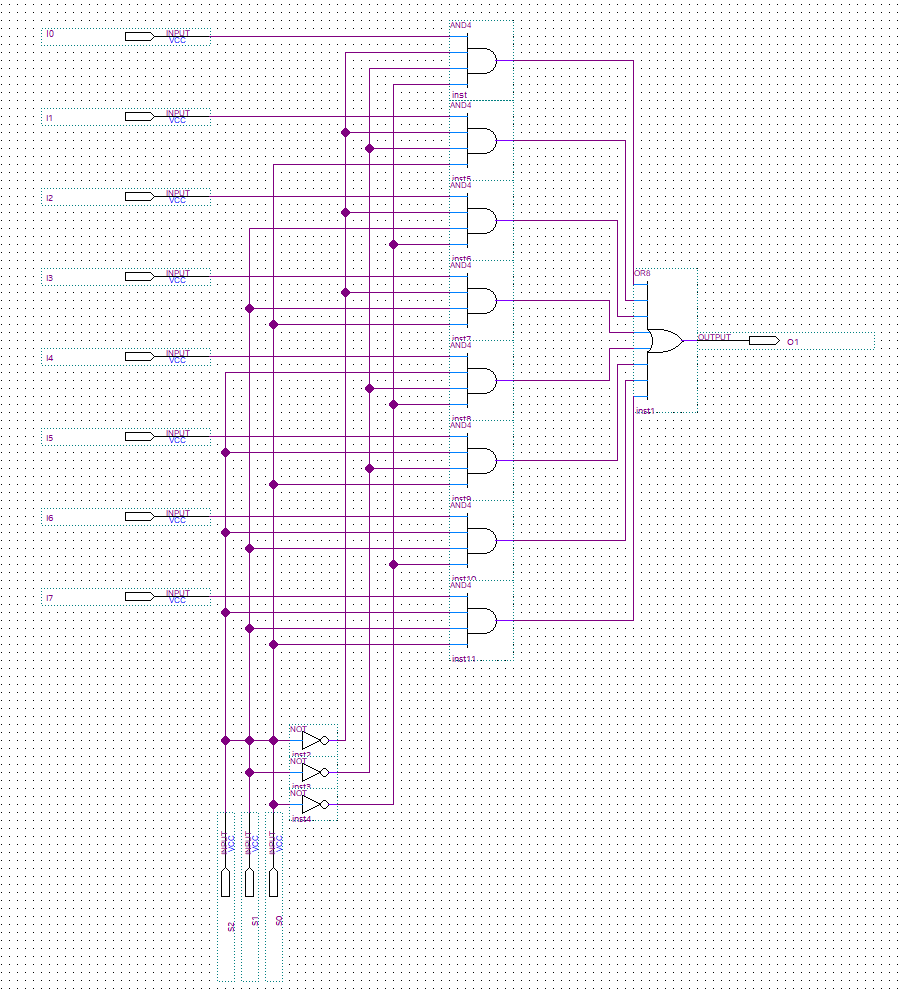
\includegraphics[width=\textwidth]{./diagrams/8x1multiplexer.png}
\end{figure}

\clearpage
\subsubsection{VHDL Code}
I also redesigned this multiplexer in VHDL using behavioral modeling.
\begin{minted}[linenos]{vhdl}
    library IEEE;
    use IEEE.std_logic_1164.all;
    
    entity multiplexer8x1v2 is
        port (
            I : in  std_logic_vector(7 downto 0);
            S : in  std_logic_vector(2 downto 0);
            O : out std_logic
        );
    end multiplexer8x1v2;
    
    architecture Behavioral of multiplexer8x1v2 is
    begin
        with S select
            O <= I(0) when "000",
                 I(1) when "001",
                 I(2) when "010",
                 I(3) when "011",
                 I(4) when "100",
                 I(5) when "101",
                 I(6) when "110",
                 I(7) when "111",
                 '0'    when others;
    end Behavioral;
\end{minted}
\clearpage

\subsection{Simulation}
I wrote VHDL to simulate both versions of the circuit.
\subsubsection{Structural Model Test Bench}

\begin{minted}{vhdl}
LIBRARY IEEE;
USE IEEE.STD_LOGIC_1164.ALL;
USE IEEE.STD_LOGIC_TEXTIO.ALL;
USE std.textio.ALL;

ENTITY tb_multiplexer8x1 IS
END tb_multiplexer8x1;

ARCHITECTURE test OF tb_multiplexer8x1 IS
    SIGNAL I0 : STD_LOGIC := '0';
    SIGNAL I1 : STD_LOGIC := '0';
    SIGNAL I2 : STD_LOGIC := '0';
    SIGNAL I3 : STD_LOGIC := '0';
    SIGNAL I4 : STD_LOGIC := '0';
    SIGNAL I5 : STD_LOGIC := '0';
    SIGNAL I6 : STD_LOGIC := '0';
    SIGNAL I7 : STD_LOGIC := '0';
    SIGNAL S2 : STD_LOGIC := '0';
    SIGNAL S1 : STD_LOGIC := '0';
    SIGNAL S0 : STD_LOGIC := '0';
    SIGNAL O1 : STD_LOGIC;

    COMPONENT mux8to1_structural IS
        PORT (
            I0 : IN STD_LOGIC;
            I2 : IN STD_LOGIC;
            I3 : IN STD_LOGIC;
            I1 : IN STD_LOGIC;
            I4 : IN STD_LOGIC;
            I5 : IN STD_LOGIC;
            I6 : IN STD_LOGIC;
            I7 : IN STD_LOGIC;
            S2 : IN STD_LOGIC;
            S1 : IN STD_LOGIC;
            S0 : IN STD_LOGIC;
            O1 : OUT STD_LOGIC
        );
    END COMPONENT;

BEGIN
    uut : mux8to1_structural
    PORT MAP(I0, I2, I3, I1, I4, I5, I6, I7, S2, S1, S0, O1);

    PROCESS
    BEGIN
        S2 <= '0';
        S1 <= '0';
        S0 <= '0';
        WAIT FOR 10 ns;
        I0 <= '1';
        WAIT FOR 10 ns;
        I0 <= '0';

        S2 <= '0';
        S1 <= '0';
        S0 <= '1';
        WAIT FOR 10 ns;
        I1 <= '1';
        WAIT FOR 10 ns;
        I1 <= '0';

        S2 <= '0';
        S1 <= '1';
        S0 <= '0';
        WAIT FOR 10 ns;
        I2 <= '1';
        WAIT FOR 10 ns;
        I2 <= '0';

        S2 <= '0';
        S1 <= '1';
        S0 <= '1';
        WAIT FOR 10 ns;
        I3 <= '1';
        WAIT FOR 10 ns;
        I3 <= '0';

        S2 <= '1';
        S1 <= '0';
        S0 <= '0';
        WAIT FOR 10 ns;
        I4 <= '1';
        WAIT FOR 10 ns;
        I4 <= '0';

        S2 <= '1';
        S1 <= '0';
        S0 <= '1';
        WAIT FOR 10 ns;
        I5 <= '1';
        WAIT FOR 10 ns;
        I5 <= '0';

        S2 <= '1';
        S1 <= '1';
        S0 <= '0';
        WAIT FOR 10 ns;
        I6 <= '1';
        WAIT FOR 10 ns;
        I6 <= '0';

        S2 <= '1';
        S1 <= '1';
        S0 <= '1';
        WAIT FOR 10 ns;
        I7 <= '1';
        WAIT FOR 10 ns;
        I7 <= '0';
    END PROCESS;
END test;

\end{minted}
This code selects inputs 0 through 7 and toggles them while they are selected to show that the output corresponds to the selected input.


\begin{figure}[h]
\caption{Output for Structural Multiplexer Test Bench}
\centering
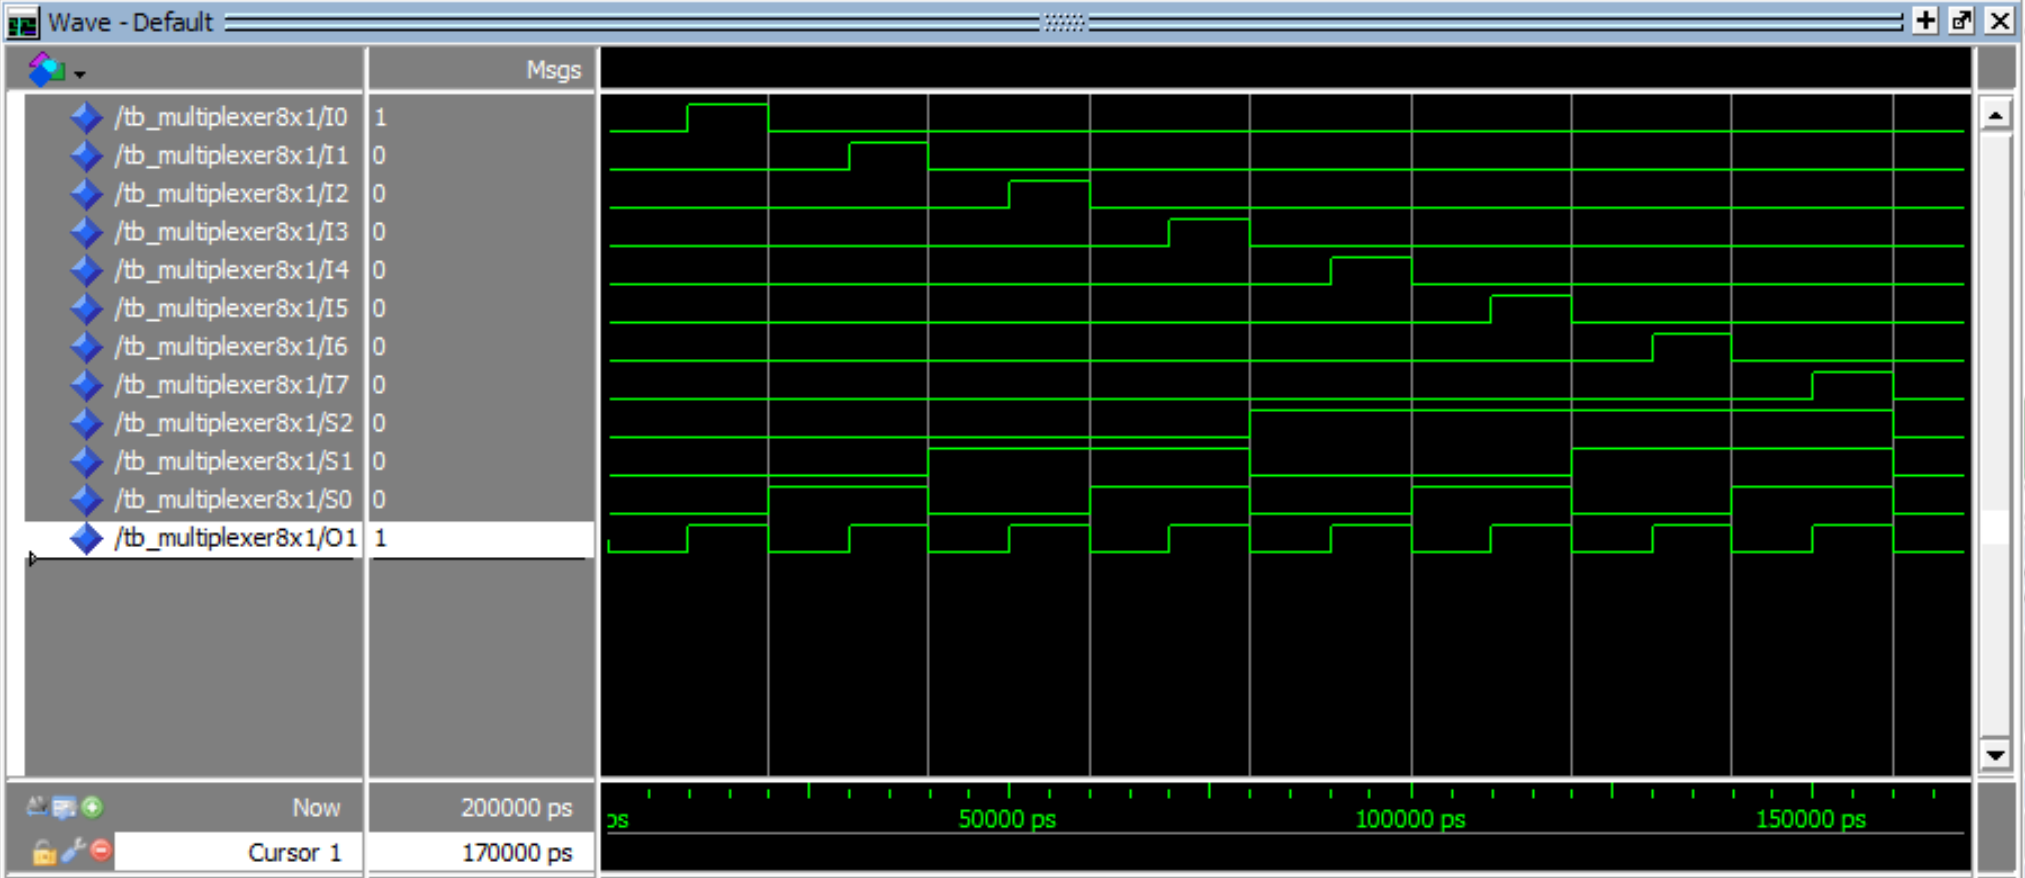
\includegraphics[width=\textwidth]{./diagrams/mux_structural.png}
\end{figure}

\clearpage
\subsubsection{Behavioral Model Test Bench}
I also wrote test bench code for the behavioral model multiplexer. This code was essentially the same as the previous test bench for the structural model. The only difference is that the inputs and the select signals were vectors.
\begin{minted}{vhdl}
    LIBRARY IEEE;
USE IEEE.STD_LOGIC_1164.ALL;
USE IEEE.STD_LOGIC_TEXTIO.ALL;
USE STD.TEXTIO.ALL;

ENTITY tb_multiplexer8x1v2 IS
END tb_multiplexer8x1v2;

ARCHITECTURE test OF tb_multiplexer8x1v2 IS
    SIGNAL I : STD_LOGIC_VECTOR(7 DOWNTO 0) := (OTHERS => '0');
    SIGNAL S : STD_LOGIC_VECTOR(2 DOWNTO 0) := "000";
    SIGNAL O : STD_LOGIC;
    COMPONENT multiplexer8x1v2 IS
        PORT (
            I : IN  STD_LOGIC_VECTOR(7 DOWNTO 0);
            S : IN  STD_LOGIC_VECTOR(2 DOWNTO 0);
            O : OUT STD_LOGIC
        );
    END COMPONENT;
BEGIN
    uut : multiplexer8x1v2
        PORT MAP (
            I => I,
            S => S,
            O => O
        );
    PROCESS
    BEGIN
        S <= "000";
        I <= (OTHERS => '0');
        WAIT FOR 10 ns;
        I(0) <= '1';
        WAIT FOR 10 ns;
        I(0) <= '0';
        S <= "001";
        I <= (OTHERS => '0');
        WAIT FOR 10 ns;
        I(1) <= '1';
        WAIT FOR 10 ns;
        I(1) <= '0';
        S <= "010";
        I <= (OTHERS => '0');
        WAIT FOR 10 ns;
        I(2) <= '1';
        WAIT FOR 10 ns;
        I(2) <= '0';
        S <= "011";
        I <= (OTHERS => '0');
        WAIT FOR 10 ns;
        I(3) <= '1';
        WAIT FOR 10 ns;
        I(3) <= '0';
        S <= "100";
        I <= (OTHERS => '0');
        WAIT FOR 10 ns;
        I(4) <= '1';
        WAIT FOR 10 ns;
        I(4) <= '0';
        S <= "101";
        I <= (OTHERS => '0');
        WAIT FOR 10 ns;
        I(5) <= '1';
        WAIT FOR 10 ns;
        I(5) <= '0';
        S <= "110";
        I <= (OTHERS => '0');
        WAIT FOR 10 ns;
        I(6) <= '1';
        WAIT FOR 10 ns;
        I(6) <= '0';
        S <= "111";
        I <= (OTHERS => '0');
        WAIT FOR 10 ns;
        I(7) <= '1';
        WAIT FOR 10 ns;
        I(7) <= '0';
        WAIT;
    END PROCESS;
END test;
\end{minted}

\begin{figure}[h]
\caption{Output for Behavioral Multiplexer Test Bench}
\centering
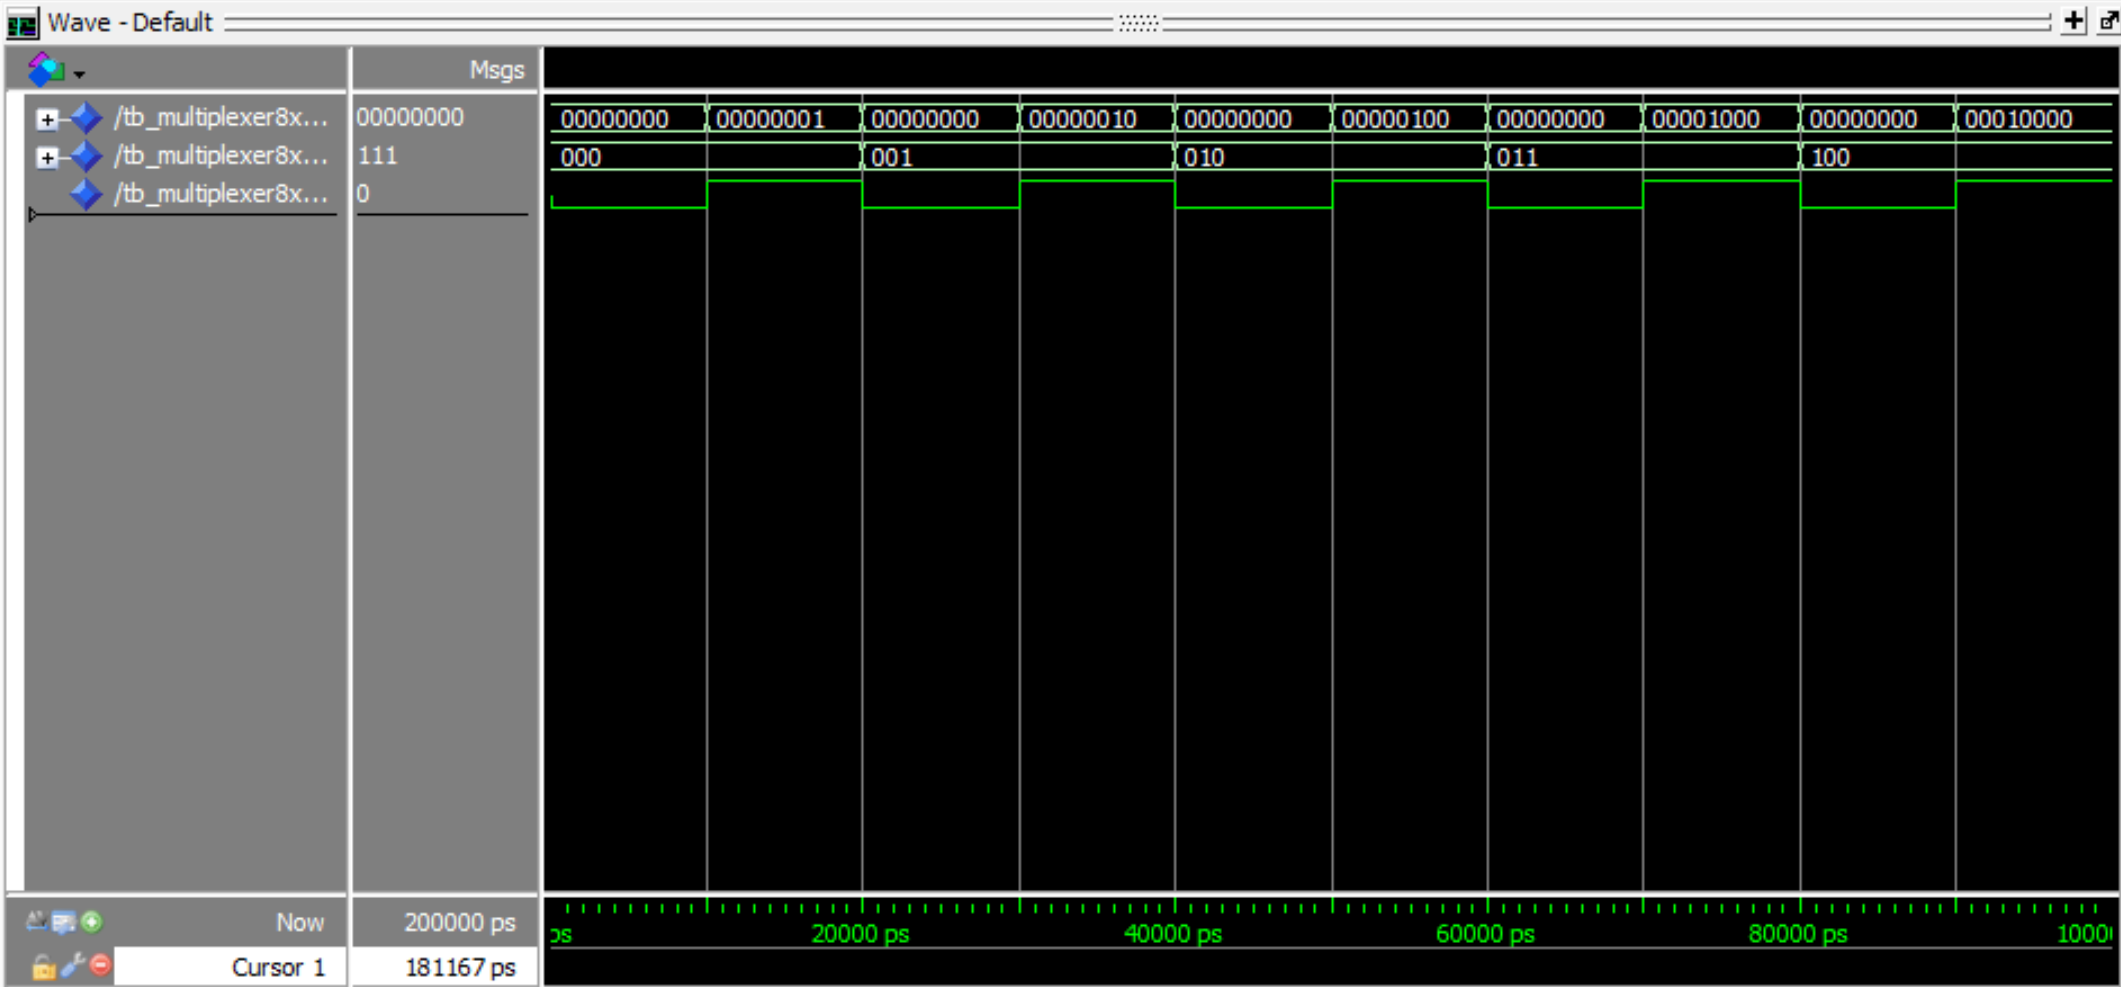
\includegraphics[width=\textwidth]{./diagrams/mux_behavioral.png}
\end{figure}
\clearpage


\section{Exercise B: 1x8 De-Multiplexer Using 1x4 and 1x2 De-Multiplexers}
\subsection{Objective}

\subsection{Functionality and Specifications}

\subsection{Simulation}
\clearpage
%-------------------- 3x8 decoder begin --------------------
\section{Exercise C: 3-to-8 Decoder}
\subsection{Objective}
The purpose of this exercise was to create a 3x8 decoder circuit from its respective combinational logic. Now having compiled and generated the relevant VHDL for the circuit one was able to simulate the circuit in action.

\subsection{Functionality and Specifications}

Here we want to describe the combinational logic functions (Boolean equations, if applicable)

\begin{figure}[h]
\caption{3x8 decoder}
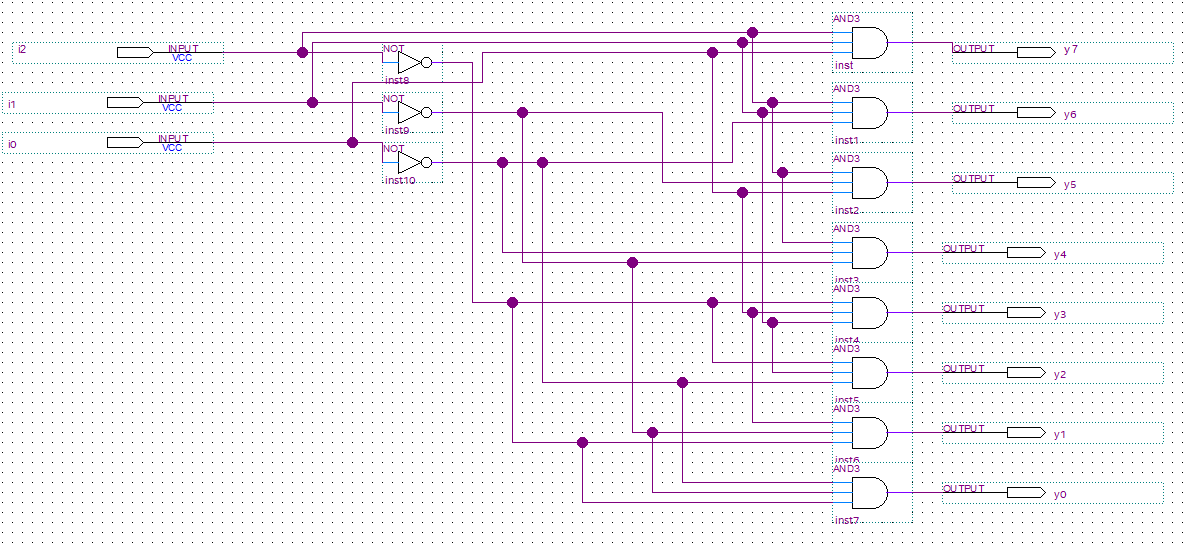
\includegraphics[width=\textwidth]{./diagrams/3x8_decoder.png}
\end{figure}
\subsubsection{VHDL Code generated from the design file}
\begin{minted}{vhdl}
    LIBRARY ieee;
    USE ieee.std_logic_1164.all;

    LIBRARY work;

    ENTITY lab_assign_1 IS
    	PORT
    	(
    		i2 :  IN  STD_LOGIC;
    		i1 :  IN  STD_LOGIC;
    		i0 :  IN  STD_LOGIC;
    		y7 :  OUT  STD_LOGIC;
    		y6 :  OUT  STD_LOGIC;
    		y5 :  OUT  STD_LOGIC;
    		y4 :  OUT  STD_LOGIC;
    		y3 :  OUT  STD_LOGIC;
    		y2 :  OUT  STD_LOGIC;
    		y1 :  OUT  STD_LOGIC;
    		y0 :  OUT  STD_LOGIC
    	);
    END lab_assign_1;

    ARCHITECTURE bdf_type OF lab_assign_1 IS

    SIGNAL	SYNTHESIZED_WIRE_12 :  STD_LOGIC;
    SIGNAL	SYNTHESIZED_WIRE_13 :  STD_LOGIC;
    SIGNAL	SYNTHESIZED_WIRE_14 :  STD_LOGIC;


    BEGIN

    y7 <= i2 AND i1 AND i0;
    y6 <= i2 AND i1 AND SYNTHESIZED_WIRE_12;

    SYNTHESIZED_WIRE_12 <= NOT(i0);
    y5 <= i2 AND SYNTHESIZED_WIRE_13 AND i0;
    y4 <= i2 AND SYNTHESIZED_WIRE_12 AND SYNTHESIZED_WIRE_13;
    y3 <= SYNTHESIZED_WIRE_14 AND i0 AND i1;
    y2 <= SYNTHESIZED_WIRE_14 AND i1 AND SYNTHESIZED_WIRE_12;
    y1 <= i0 AND SYNTHESIZED_WIRE_13 AND SYNTHESIZED_WIRE_14;
    y0 <= SYNTHESIZED_WIRE_12 AND SYNTHESIZED_WIRE_13 AND SYNTHESIZED_WIRE_14;

    SYNTHESIZED_WIRE_14 <= NOT(i2);
    SYNTHESIZED_WIRE_13 <= NOT(i1);
    END bdf_type;

\end{minted}

\subsubsection{VHDL code for Test bench}
\begin{minted}{vhdl}
    library IEEE;
    use IEEE.STD_LOGIC_1164.ALL;
    use IEEE.STD_LOGIC_TEXTIO.ALL;
    use std.textio.all;

    entity tb_3x8_decoder is
    end tb_3x8_decoder;

    architecture test of tb_3x8_decoder is
        signal i2 :  STD_LOGIC;
        signal i1 :  STD_LOGIC;
        signal i0 :  STD_LOGIC;
        signal y7 :  STD_LOGIC;
        signal y6 :  STD_LOGIC;
        signal y5 :  STD_LOGIC;
        signal y4 :  STD_LOGIC;
        signal y3 :  STD_LOGIC;
        signal y2 :  STD_LOGIC;
        signal y1 :  STD_LOGIC;
        signal y0 :  STD_LOGIC;

        component lab_assign_1
    	Port
    	(
    		i2 :  IN  STD_LOGIC;
    		i1 :  IN  STD_LOGIC;
    		i0 :  IN  STD_LOGIC;
    		y7 :  OUT  STD_LOGIC;
    		y6 :  OUT  STD_LOGIC;
    		y5 :  OUT  STD_LOGIC;
    		y4 :  OUT  STD_LOGIC;
    		y3 :  OUT  STD_LOGIC;
    		y2 :  OUT  STD_LOGIC;
    		y1 :  OUT  STD_LOGIC;
    		y0 :  OUT  STD_LOGIC
    	);
        end component;

    begin
        uut: lab_assign_1 port map(i2, i1, i0, y7, y6, y5, y4, y3, y2, y1,y0);
        PROCESS
        BEGIN
            i2 <= '0';
            i1 <= '0';
            i0 <= '0';
            WAIT for 10 ns;
            i0 <= '1';
            WAIT for 10 ns;
            i1 <= '1';
            i0 <= '0';
            WAIT for 10 ns;
            i0 <= '1';
            WAIT for 10 ns;
            i2 <= '1';
            i1 <= '0';
            i0 <= '0';
            WAIT for 10 ns;
            i0 <= '1';
            WAIT for 10 ns;
            i1 <= '1';
            i0 <= '0';
            WAIT for 10 ns;
            i0 <= '1';
            WAIT for 10 ns;
        END PROCESS;

    end test;
\end{minted}

\subsection{Simulation}
\begin{figure}[h]
\caption{3x8 decoder wave simulation}
\centering
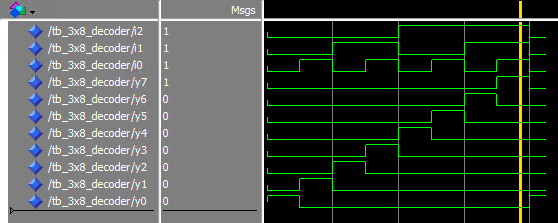
\includegraphics[width=\textwidth]{./diagrams/3x8_simulation.png}
\end{figure}
%-------------------- 3x8 decoder END --------------------
\clearpage
%-------------------- 8x3 p-encoder begin --------------------
\section{Exercise D: 8-to-3 Priority Encoder}
\subsection{Objective}
The purpose of this exercise was to create a 8x3 priority encoder circuit from its respective combinational logic. Now having compiled and generated the relevant VHDL for the circuit one was able to simulate the circuit in action. Thus resulting in a better understanding of designing a 8x3 priority encoder circuit from its respective combinational equation, and testing that created circuit.

\subsection{Functionality and Specifications}
\[
\begin{aligned}
Y_2 &= D_7 + D_6 + D_5 + D_4,\\[1mm]
Y_1 &= D_7 + D_6 + \overline{D_7 + D_6}\,(D_3 + D_2),\\[1mm]
Y_0 &= D_7 + \overline{D_7 + D_6}\,D_5 + \overline{D_7 + D_6 + D_5}\,D_3 + \overline{D_7 + D_6 + D_5 + D_4}\,D_1.
\end{aligned}
\]

Here we want to describe the combinational logic functions (our equations essentially )

\begin{figure}[h]
\caption{8x3 priority encoder}
\centering
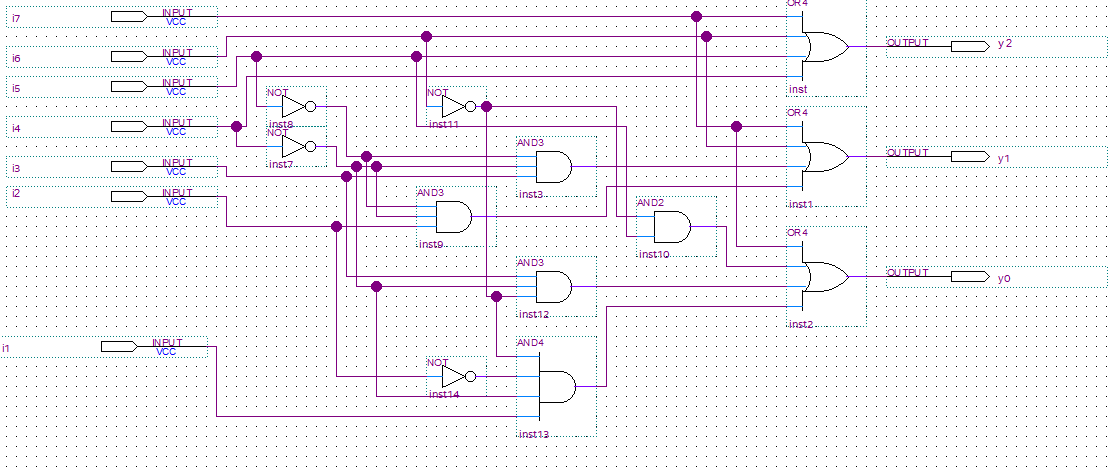
\includegraphics[width=\textwidth]{./diagrams/8x3_penc_design.png}
\end{figure}
{VHDL code generated from design file}
\begin{minted}{vhdl}
    LIBRARY ieee;
    USE ieee.std_logic_1164.all;

    LIBRARY work;

    ENTITY \8x3_p_enc\ IS
    	PORT
    	(
    		i2 :  IN  STD_LOGIC;
    		i1 :  IN  STD_LOGIC;
    		i3 :  IN  STD_LOGIC;
    		i4 :  IN  STD_LOGIC;
    		i5 :  IN  STD_LOGIC;
    		i6 :  IN  STD_LOGIC;
    		i7 :  IN  STD_LOGIC;
    		y2 :  OUT  STD_LOGIC;
    		y1 :  OUT  STD_LOGIC;
    		y0 :  OUT  STD_LOGIC
    	);
    END \8x3_p_enc\;

    ARCHITECTURE bdf_type OF \8x3_p_enc\ IS

    SIGNAL	SYNTHESIZED_WIRE_0 :  STD_LOGIC;
    SIGNAL	SYNTHESIZED_WIRE_1 :  STD_LOGIC;
    SIGNAL	SYNTHESIZED_WIRE_15 :  STD_LOGIC;
    SIGNAL	SYNTHESIZED_WIRE_16 :  STD_LOGIC;
    SIGNAL	SYNTHESIZED_WIRE_6 :  STD_LOGIC;
    SIGNAL	SYNTHESIZED_WIRE_8 :  STD_LOGIC;
    SIGNAL	SYNTHESIZED_WIRE_9 :  STD_LOGIC;
    SIGNAL	SYNTHESIZED_WIRE_10 :  STD_LOGIC;
    SIGNAL	SYNTHESIZED_WIRE_17 :  STD_LOGIC;


    BEGIN



    y2 <= i7 OR i5 OR i4 OR i6;


    y1 <= i7 OR SYNTHESIZED_WIRE_0 OR SYNTHESIZED_WIRE_1 OR i6;


    SYNTHESIZED_WIRE_10 <= SYNTHESIZED_WIRE_15 AND i5;


    SYNTHESIZED_WIRE_15 <= NOT(i6);



    SYNTHESIZED_WIRE_8 <= i3 AND SYNTHESIZED_WIRE_16 AND SYNTHESIZED_WIRE_15;


    SYNTHESIZED_WIRE_9 <= SYNTHESIZED_WIRE_15 AND SYNTHESIZED_WIRE_6 AND SYNTHESIZED_WIRE_16 AND i1;


    SYNTHESIZED_WIRE_6 <= NOT(i2);



    y0 <= i7 OR SYNTHESIZED_WIRE_8 OR SYNTHESIZED_WIRE_9 OR SYNTHESIZED_WIRE_10;


    SYNTHESIZED_WIRE_0 <= SYNTHESIZED_WIRE_17 AND SYNTHESIZED_WIRE_16 AND i3;


    SYNTHESIZED_WIRE_16 <= NOT(i4);



    SYNTHESIZED_WIRE_17 <= NOT(i5);



    SYNTHESIZED_WIRE_1 <= SYNTHESIZED_WIRE_17 AND SYNTHESIZED_WIRE_16 AND i2;


    END bdf_type;

\end{minted}

\subsubsection{VHDL code for Test bench}
\begin{minted}{vhdl}
    library IEEE;
    use IEEE.STD_LOGIC_1164.ALL;
    use IEEE.STD_LOGIC_TEXTIO.ALL;
    use std.textio.all;

    entity tb_8x3_p_encoder is
    end tb_8x3_p_encoder;

    architecture test of tb_8x3_p_encoder is
        signal i1 : STD_LOGIC;
        signal i2 : STD_LOGIC;
        signal i3 : STD_LOGIC;
        signal i4 : STD_LOGIC;
        signal i5 : STD_LOGIC;
        signal i6 : STD_LOGIC;
        signal i7 : STD_LOGIC;
        signal y2 : STD_LOGIC;
        signal y1 : STD_LOGIC;
        signal y0 : STD_LOGIC;

        component \8x3_p_enc\
            Port ( i1 : in STD_LOGIC;
                   i2 : in STD_LOGIC;
                   i3 : in STD_LOGIC;
                   i4 : in STD_LOGIC;
                   i5 : in STD_LOGIC;
                   i6 : in STD_LOGIC;
                   i7 : in STD_LOGIC;
                   y2 : out STD_LOGIC;
                   y1 : out STD_LOGIC;
    	       y0 : out STD_LOGIC);
        end component;

    begin
        uut: \8x3_p_enc\ port map(i1, i2, i3, i4, i5, i6, i7, y2, y1, y0);
        PROCESS
        BEGIN
    	-- No inputs active
            i1 <= '0';
            i2 <= '0';
            i3 <= '0';
            i4 <= '0';
            i5 <= '0';
            i6 <= '0';
            i7 <= '0';
            WAIT for 20 ns;
            -- i1 active
            i1 <= '1';
            i2 <= '0';
            i3 <= '0';
            i4 <= '0';
            i5 <= '0';
            i6 <= '0';
            i7 <= '0';
            WAIT for 20 ns;
            -- i2 active
            i1 <= '0';
            i2 <= '1';
            i3 <= '0';
            i4 <= '0';
            i5 <= '0';
            i6 <= '0';
            i7 <= '0';
            WAIT for 20 ns;
            -- i3 active
            i1 <= '0';
            i2 <= '0';
            i3 <= '1';
            i4 <= '0';
            i5 <= '0';
            i6 <= '0';
            i7 <= '0';
            WAIT for 20 ns;
            -- i4 active
            i1 <= '0';
            i2 <= '0';
            i3 <= '0';
            i4 <= '1';
            i5 <= '0';
            i6 <= '0';
            i7 <= '0';
            WAIT for 20 ns;
            -- i5 active
            i1 <= '0';
            i2 <= '0';
            i3 <= '0';
            i4 <= '0';
            i5 <= '1';
            i6 <= '0';
            i7 <= '0';
            WAIT for 20 ns;
            -- i6 active
            i1 <= '0';
            i2 <= '0';
            i3 <= '0';
            i4 <= '0';
            i5 <= '0';
            i6 <= '1';
            i7 <= '0';
            WAIT for 20 ns;
            -- i7 active
            i1 <= '0';
            i2 <= '0';
            i3 <= '0';
            i4 <= '0';
            i5 <= '0';
            i6 <= '0';
            i7 <= '1';
            WAIT for 20 ns;
            -- multiple active, output should be: (Highest priority, i7)
            i1 <= '0';
            i2 <= '0';
            i3 <= '1';
            i4 <= '0';
            i5 <= '1';
            i6 <= '0';
            i7 <= '1';
            WAIT for 20 ns;
            -- multiple active, output should be: (Highest priority, i6)
            i1 <= '1';
            i2 <= '1';
            i3 <= '1';
            i4 <= '1';
            i5 <= '0';
            i6 <= '1';
            i7 <= '0';
            WAIT for 20 ns;
            -- multiple active, output should be: (Highest priority, i5)
            i1 <= '1';
            i2 <= '1';
            i3 <= '1';
            i4 <= '1';
            i5 <= '1';
            i6 <= '0';
            i7 <= '0';
            WAIT for 20 ns;
            -- multiple active, output should be: (Highest priority, i4)
            i1 <= '1';
            i2 <= '1';
            i3 <= '1';
            i4 <= '1';
            i5 <= '0';
            i6 <= '0';
            i7 <= '0';
            WAIT for 20 ns;
            -- multiple active, output should be: (Highest priority, i3)
            i1 <= '1';
            i2 <= '1';
            i3 <= '1';
            i4 <= '0';
            i5 <= '0';
            i6 <= '0';
            i7 <= '0';
            WAIT for 20 ns;
            -- multiple active, output should be: (Highest priority, i2)
            i1 <= '1';
            i2 <= '1';
            i3 <= '0';
            i4 <= '0';
            i5 <= '0';
            i6 <= '0';
            i7 <= '0';
            WAIT for 20 ns;

        END PROCESS;

    end test;

\end{minted}


\subsection{Simulation}
In this simulation part regarding the (Draw truth tables based on the waveforms.) part we just compare the wave form against the
\begin{figure}[h]
\caption{8x3 priority encoder wave graph}
\centering
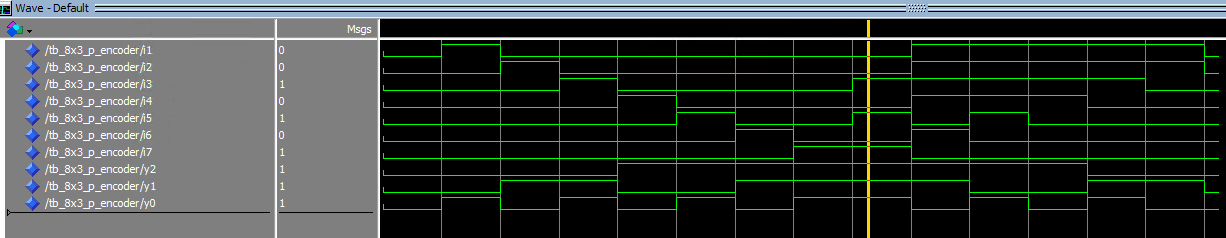
\includegraphics[width=\textwidth]{./diagrams/8x3_p_enc_simulation.png}
\end{figure}

%-------------------- 8x3 p-encoder END --------------------
\clearpage
%-------------------- SR latch & Flip flop begin --------------------
\section{Exercise E: Set-Reset Flip-Flop \& D Flip-Flop (Positive Edge Trigger)}
\subsection{Objective}
Up until now we've modeled both the set reset flip-flop and the D flip-flop using logic gates. The goal of this section was to instead model both flip-flops behaviorally in VHDL.
\subsection{Functionality and Specifications}
\subsubsection{Set-Reset Flip-Flop Truth Table}
The following truth table describes the behavior of our SR flip-flop.
\begin{center}
    \begin{tabular}{|c|c|c|c|c|}
        \hline
        CLK & R & S & Q & $\overline{Q}$ \\ 
        \hline
        0 & X & X & NO CHG & NO CHG \\ 
        1 & X & X & NO CHG & NO CHG \\ 
        $\downarrow$ & X & X & NO CHG & NO CHG \\ 
        $\uparrow$ & 0 & 0 & NO CHG & NO CHG \\ 
        $\uparrow$ & 0 & 1 & SET & RESET \\ 
        $\uparrow$ & 1 & 0 & RESET & SET \\ 
        $\uparrow$ & 1 & 1 & ILLEGAL & ILLEGAL \\ 
        \hline
    \end{tabular}
\end{center}
During the rising edge of the clock when the clock transitions from 0 to 1, the outputs \( Q \) and \( \overline{Q} \) update according to these rules:
\begin{itemize}
\item If \( S = 1 \), then the flip-flop is set: \( Q \) becomes 1 and \( \overline{Q} \) becomes 0.
\item If \( R = 1 \), then the flip-flop is reset: \( Q \) becomes 0 and \( \overline{Q} \) becomes 1.
\item If both \( R \) and \( S \) are inactive (i.e., \( R = 0 \) and \( S = 0 \)), the outputs remain unchanged. 
\item The condition where both \( R = 1 \) and \( S = 1 \) is considered illegal for this circuit.
\end{itemize}
\clearpage
\subsubsection{D Flip-Flop Truth Table}



The following truth table illustrates the behavior of the D flip-flop:

\begin{center}
    \renewcommand{\arraystretch}{1.5}
    \begin{tabular}{|c|c|c|}
        \hline
        CLK & D & \(Q\) \\ 
        \hline
        0 & X & NO CHG  \\ 
        1 & X & NO CHG  \\ 
        \(\downarrow\) & X & NO CHG \\ 
        \(\uparrow\) & 0 & RESET  \\ 
        \(\uparrow\) & 1 & SET  \\ 
        \hline
    \end{tabular}
\end{center}
Here, \(Q\) changes to be equal to \(D\) whenever the clock is rising.
\subsubsection{Set-Reset Flip-Flop VHDL Code}
\begin{minted}[linenos]{vhdl}
LIBRARY ieee;
USE ieee.std_logic_1164.ALL;

ENTITY sr_flip_flop IS
	PORT (
		s : IN STD_LOGIC;
		r : IN STD_LOGIC;
		clk : IN STD_LOGIC;
		q : OUT STD_LOGIC;
		qc : OUT STD_LOGIC
	);
END sr_flip_flop;

ARCHITECTURE behavior OF sr_flip_flop IS
	SIGNAL S_Q : STD_LOGIC;
BEGIN
	q <= S_Q;
	qc <= NOT S_Q;
	PROCESS (clk)
	BEGIN
		IF rising_edge(clk) THEN
			IF s = '1' AND r = '0' THEN
				S_Q <= '1';
			ELSIF s = '0' AND r = '1' THEN
				S_Q <= '0';
			END IF;
		END IF;
	END PROCESS;
END behavior;
\end{minted}

\subsubsection{D Flip-Flop VHDL Code}
\begin{minted}[linenos]{vhdl}
    library IEEE;
use IEEE.STD_LOGIC_1164.ALL;

entity d_flip_flop is
    Port (
        D   : in STD_LOGIC;  -- Data input
        CLK : in STD_LOGIC;  -- Clock signal
        Q   : out STD_LOGIC  -- Output
    );
end d_flip_flop;

architecture Behavioral of d_flip_flop is
begin
    process(CLK)
    begin
        if rising_edge(CLK) then
            Q <= D;
        end if;
    end process;
end Behavioral;
\end{minted}
\subsection{Simulation}
\subsubsection{Set-Reset Flip-Flop Test Bench}
The following is the test match code for the set reset flip-flop.
\begin{minted}[linenos]{vhdl}
LIBRARY IEEE;
USE IEEE.STD_LOGIC_1164.ALL;

ENTITY tb_sr_flip_flop IS
END tb_sr_flip_flop;

ARCHITECTURE testbench OF tb_sr_flip_flop IS
    SIGNAL S : STD_LOGIC := '0'; -- Signal for data input
    SIGNAL R : STD_LOGIC := '0'; -- Signal for data input
    SIGNAL CLK : STD_LOGIC := '0'; -- Clock signal
    SIGNAL Q : STD_LOGIC; -- Output signal
    SIGNAL QC : STD_LOGIC; -- Output signal
BEGIN
    -- Instantiate the SR Flip-Flop
    uut : ENTITY work.sr_flip_flop
        PORT MAP(S, R, CLK, Q, QC);

        -- Clock Generation Process
        CLK_Process : PROCESS
        BEGIN
            WHILE now < 100 ns LOOP -- Limit the clock process to 100 ns
            CLK <= '0';
            WAIT FOR 5 ns;
            CLK <= '1';
            WAIT FOR 5 ns;
        END LOOP;
        WAIT; -- Stops the clock process after 100 ns
        END PROCESS;

        -- Test Process
        Stimulus_Process : PROCESS
        BEGIN
            R <= '1';
            WAIT FOR 20 ns;
            R <= '0';
            WAIT FOR 20 ns;

            S <= '1';
            WAIT FOR 20 ns;
            S <= '0';
            WAIT FOR 20 ns;

            R <= '1';
            WAIT FOR 20 ns;
            R <= '0';
            WAIT FOR 20 ns;

            WAIT;

    
        END PROCESS;
END testbench;
\end{minted}
\clearpage
Here is the output for this code. In the waveform, you can see that the output for Q and QC only get updated on the rising edge of the clock when either S or R are set according to the rules outlined earlier. \\
\begin{figure}[H]
\caption{Output for Set-Reset Flip-Flop Test Bench}
\centering
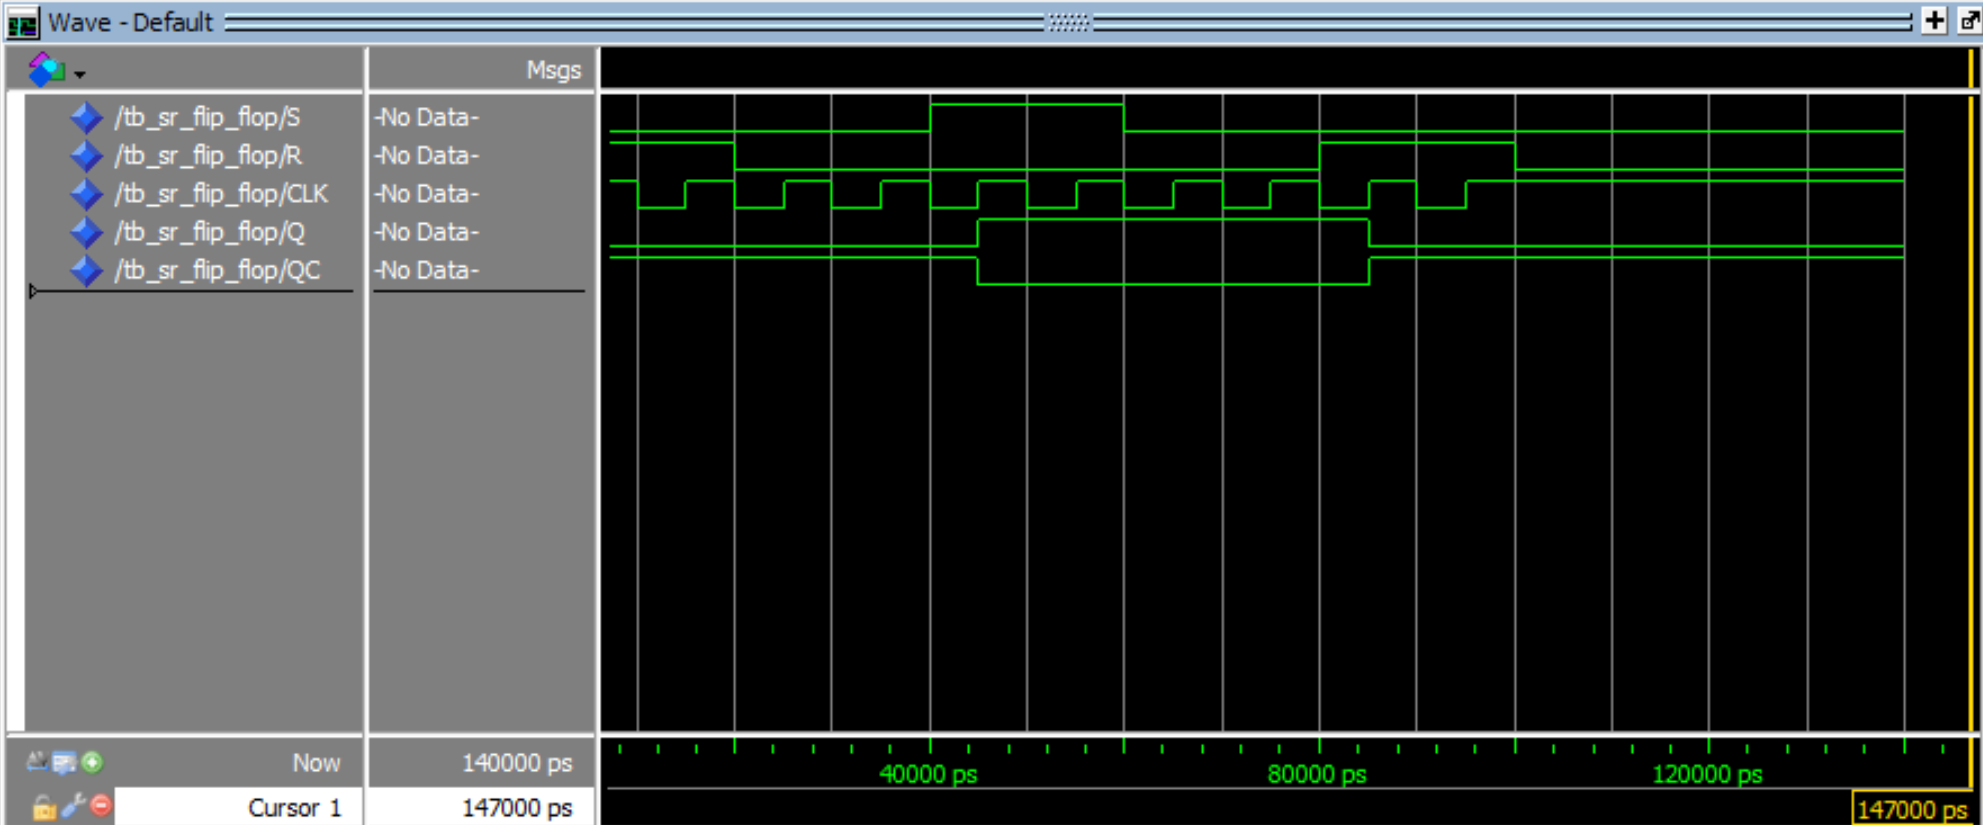
\includegraphics[width=\textwidth]{./diagrams/sr_flipflop.png}
\end{figure}

\subsubsection{D Flip-Flop Test Bench}
\begin{minted}[linenos]{vhdl}
library IEEE;
use IEEE.STD_LOGIC_1164.ALL;

entity tb_d_flip_flop is
end tb_d_flip_flop;

architecture Testbench of tb_d_flip_flop is
    signal D   : STD_LOGIC := '0'; -- Signal for data input
    signal CLK : STD_LOGIC := '0'; -- Clock signal
    signal Q   : STD_LOGIC;        -- Output signal
begin
    -- Instantiate the D Flip-Flop
    uut: entity work.d_flip_flop
        Port Map ( D, CLK, Q );

    -- Clock Generation Process
    CLK_Process: process
    begin
        while now < 100 ns loop  -- Limit the clock process to 100 ns
            CLK <= '0';
            wait for 5 ns;
            CLK <= '1';
            wait for 5 ns;
        end loop;
        wait; -- Stops the clock process after 100 ns
    end process;

    -- Test Process
    Stimulus_Process: process
    begin
        D <= '1';
        wait for 20 ns;
        D <= '0';
        wait for 20 ns;

        D <= '1';
        wait for 20 ns;
        D <= '0';
        wait for 20 ns;

        D <= '1';
        wait for 20 ns;
        D <= '0';
        wait for 20 ns;

        wait;

    end process;
end Testbench;
\end{minted}

This code results in the waveform shown in Figure 9.
\begin{figure}[H]
\caption{Output for D Flip-Flop test bench.}
\centering
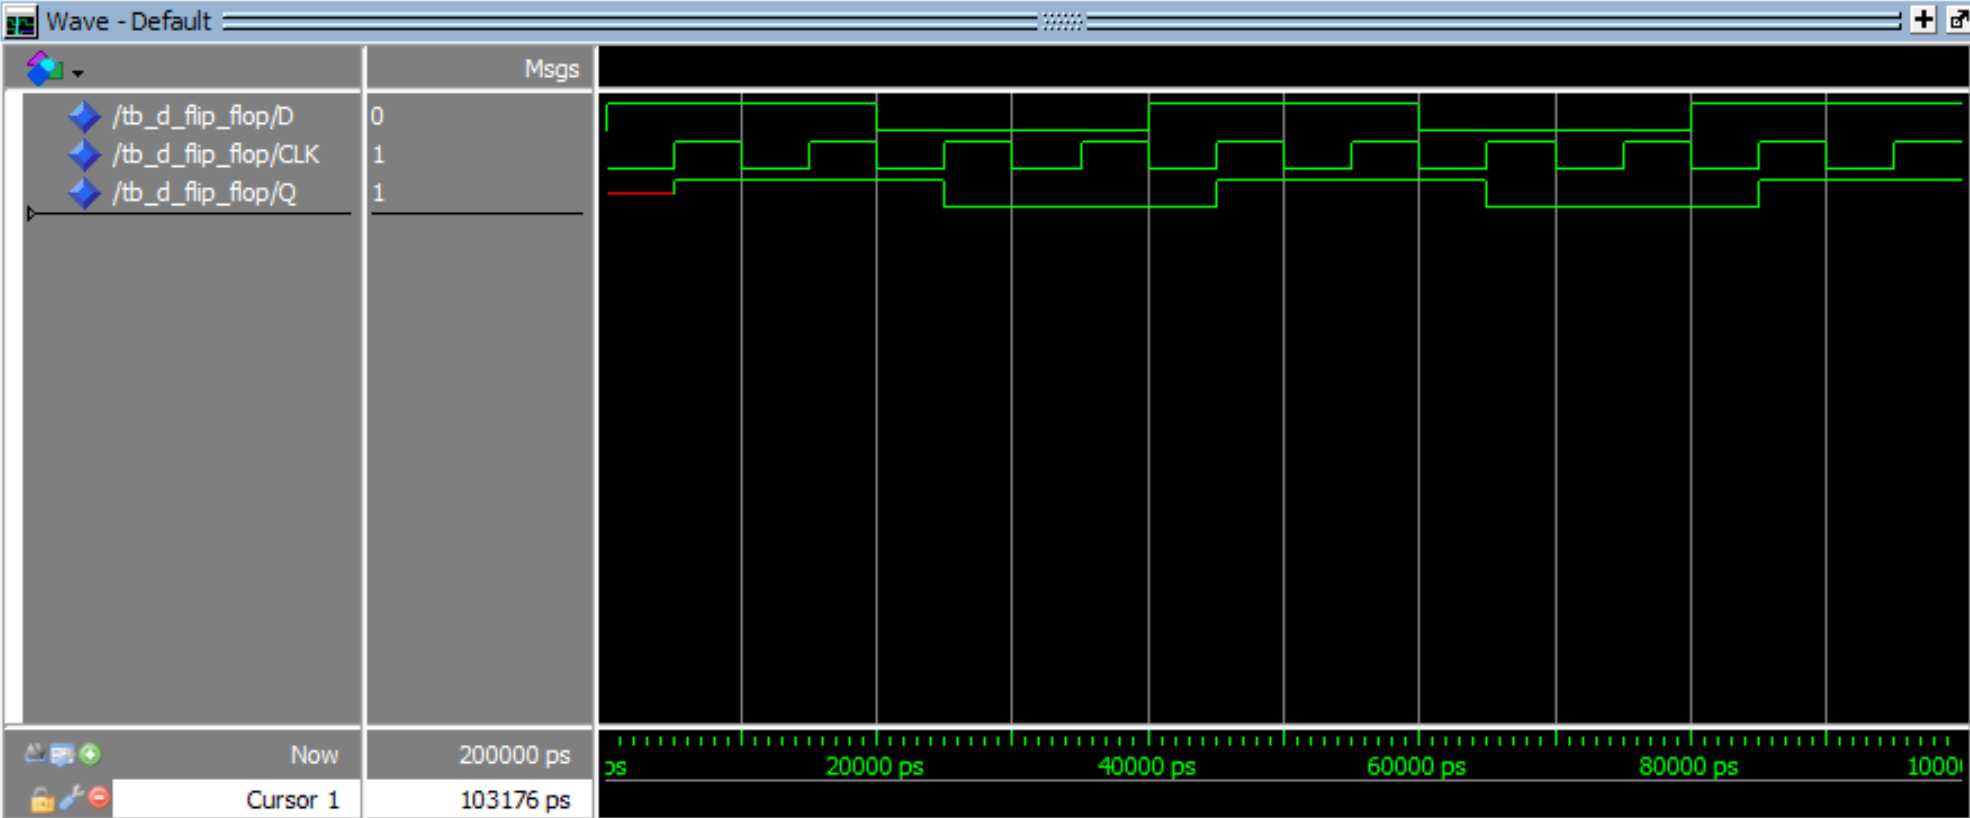
\includegraphics[width=\textwidth]{./diagrams/d_flipflop.png}
\end{figure}
Here, the value of Q gets updated to match the value of D whenever the clock rises.
\newpage
\subsection{Differences between the Set-Reset Flip-Flop and the D Flip-Flop}
The D flip-flop is very simple: on a rising clock edge, 
\[
Q \gets D.
\]

In contrast, the SR flip-flop responds on the rising clock edge as follows:
\begin{itemize}
    \item If \( S = 1 \), then \( Q = 1 \) and \( \overline{Q} = 0 \).
    \item If \( R = 1 \), then \( Q = 0 \) and \( \overline{Q} = 1 \).
    \item If \( S = 0 \) and \( R = 0 \), then \( Q \) remains unchanged.
\end{itemize}
\section{Conclusions}


We learned about the VHDL language, including data types, input/output/intermediate signals, and its parallel execution model. We observed parallel computation outside processes and sequential operations within processes.

Initially, we struggled with \texttt{when} and \texttt{if} statements, learning through experimentation that \texttt{when} is for outside processes and \texttt{if} for inside processes.  We also learned processes re-evaluate outputs only when specified inputs change.

We recognized that VHDL's standard logic datatype can hold values other than '0' and '1' such as uninitialized, unknown, and 'don't care' states, which can allow the compiler to create more efficient designs.

We also learned the difference between structural vs. behavioral modeling. Structural modeling is akin to wiring components inside of code, while behavioral modeling describes logic for the compiler to implement.

Challenges included ModelSim and Intel Quartus' project structure, making file management cumbersome. ModelSim's file update behavior, requiring manual saving and recompilation unlike IDEs like IntelliJ IDEA, caused inefficiencies and frustration as well.
\end{document}